\begin{titlepage}
% \newgeometry{left=1cm,bottom=0.8cm,right=0.8cm,top=0.8cm}
% \usetikzlibrary{mindmap,backgrounds}
\thispagestyle{empty}
% \vspace*{1em}
{\kaishu 北京化工大学本科毕业论文(设计)}
\vspace*{2cm}
\begin{flushright}
 \zihao{3}\heiti 微生物土壤运移模型的求解\\[0.8em]及仿真软件编制\\[0.8em]
\end{flushright}
\vspace{2\baselineskip}
\begin{flushleft}
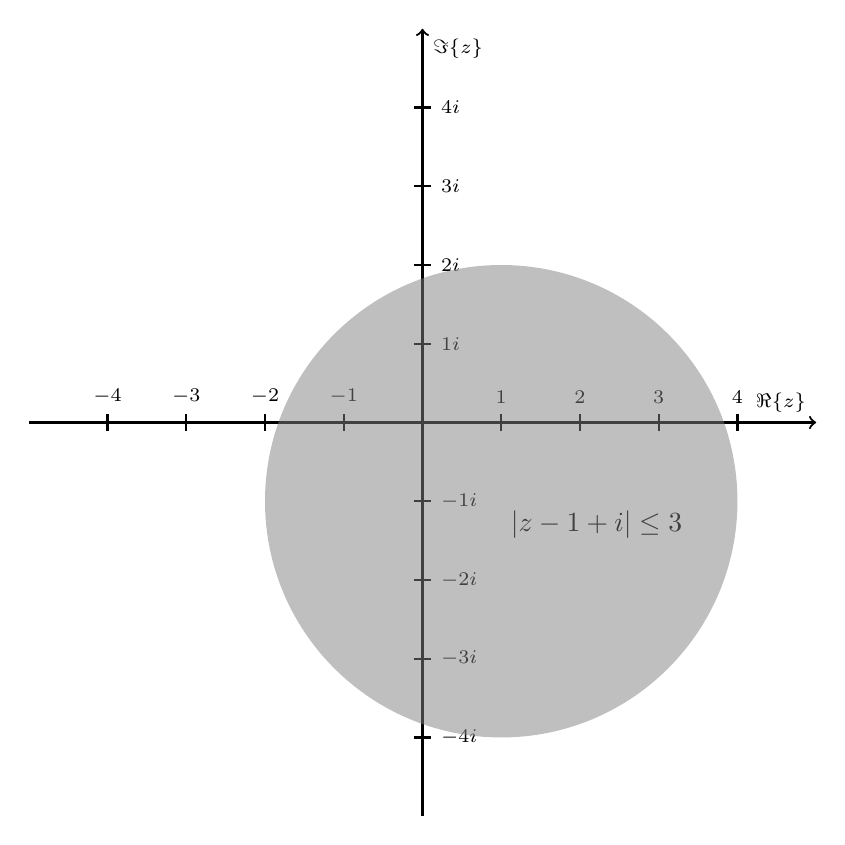
\begin{tikzpicture}
\begin{scope}[thick,font=\scriptsize]
    % Axes:
    % Are simply drawn using line with the `->` option to make them arrows:
    % The main labels of the axes can be places using `node`s:
    \draw [->] (-5,0) -- (5,0) node [above left]  {$\Re\{z\}$};
    \draw [->] (0,-5) -- (0,5) node [below right] {$\Im\{z\}$};
    % Axes labels:
    % Are drawn using small lines and labeled with `node`s. The placement can be set using options
    \iffalse% Single
    % If you only want a single label per axis side:
    \draw (1,-3pt) -- (1,3pt)   node [above] {$1$};
    \draw (-1,-3pt) -- (-1,3pt) node [above] {$-1$};
    \draw (-3pt,1) -- (3pt,1)   node [right] {$i$};
    \draw (-3pt,-1) -- (3pt,-1) node [right] {$-i$};
    \else% Multiple
    % If you want labels at every unit step:
    \foreach \n in {-4,...,-1,1,2,...,4}{%
        \draw (\n,-3pt) -- (\n,3pt)   node [above] {$\n$};
        \draw (-3pt,\n) -- (3pt,\n)   node [right] {$\n i$};
    }
    \fi
    \end{scope}
    % The circle is drawn with `(x,y) circle (radius)`
    % You can draw the outer border and fill the inner area differently.
    % Here I use gray, semitransparent filling to not cover the axes below the circle
    \path [draw=none,fill=gray,semitransparent] (+1,-1) circle (3);
    % Place the equation into the circle:
    \node [below right,darkgray] at (+1,-1) {$|z-1+i| \leq 3$};
\end{tikzpicture}
\end{flushleft}
\vfill
\begin{flushright}
\zihao{-4}\kaishu 陆秋文\quad\\[0.8em]
指导教师\quad 周\quad 延
\end{flushright}
\end{titlepage}
\clearpage{\pagestyle{empty}\cleardoublepage}
% \restoregeometry